\subsubsection{Gate-Treiber}
\label{subsubsec:Gate-Treiber}

%Nebst dem TMC4671, welcher für die Ansteuerung benötigt wird, braucht es für die Magnetisierung der Spulen des BLDC-Motors eine Schaltlogik. Dabei Handelt es sich um den TMC6200. Dieser ist eine umfangreiche Ergänzung zum TMC4671. Auf den TMC6200 und weitere benötigte Komponenten wird im folgenden eingegangen.
%\subsubsection{Problem}\label{subsubsec:Problem_TMC6200}

Die Gate-CTRL-Signale werden vom Gate-Treiber aufbereitet. Das entsprechende Bauteil ist der TMC6200. Er verarbeitet die Signale so, dass die H-Brücke angesteuert werden kann. Die H-Brücke besteht aus sechs MOSFETs, die gemäss den Gate-CTRL-Signalen die Zwischenkreisspannung (48VDC) schalten.
%Um einen MOSFET in einen leitenden Zustand zu bringen, muss das Gate des MOSFET's mit einer elektrischen Ladung gefüllt werden. Während dieses Vorgangs verhält sich das Gate kapazitiv. Dies bedeutet, dass bei jedem Schaltvorgang Ströme fliessen.

Um ein optimales Schaltverhalten zu erreichen, die Umschaltverluste zu verkleinern und somit die daraus entstehende Abwärme zu verringern, ist es vorteilhaft, die Gates so schnell wie möglich zu laden und zu entladen. Ein Gate-Treiber löst dieses Problem, indem die benötigte Energie zur Verfügung stellt. Ausserdem hebt der Gate-Treiber mit einer Bootstrap-Schaltung die Gate-Spannungen der High-Level-MOSFETS auf die Motorspannung plus Gatespannung, damit der MOSFET sicher durchschaltet.

Das Blockdiagramm und eine Beispielschaltung befinden sich im Anhang Kapitel \ref{Appendix:Schaltung_TMC6200} und \ref{Appendix:Blockdiagramm_TMC6200}. Das Blockdiagramm zeigt, dass der Gate-Treiber aus einer Treiber-Logik für den Motor, einem SPI-/Pinsettings-Interface, einer Diagnosenlogik, Strommessschaltung und diversen unterstützenden Schaltungen wie Gate-Spannungsversorgung besteht. Weiter hat der ausgewählte Gate-Treiber folgende Features integriert:
\begin{itemize}
\item Strommessung und -Verstärkung
\item Kurzschlussdetektion
\item Schaltkontrolle
\item Thermische Begrenzung
\end{itemize}

\paragraph{Schema}\mbox{}

Der Treiber und dessen Beschaltung ist als Breakoutboard erhältlich. Daran sind diverse Anschlussmöglichkeiten vorhanden. In Abbildung \ref{fig:Schema_Gate_Treiber} ist zu sehen, welche Pins verwendet werden:

\begin{itemize}
\item SPI Input
\item Phasenströme Input und Output
\item Motorspannung Input
\item Gate-HIGH und -Low-Signale Output
\item Messung Schaltspannung Input
\end{itemize}

\begin{figure}[H]
	\centering
	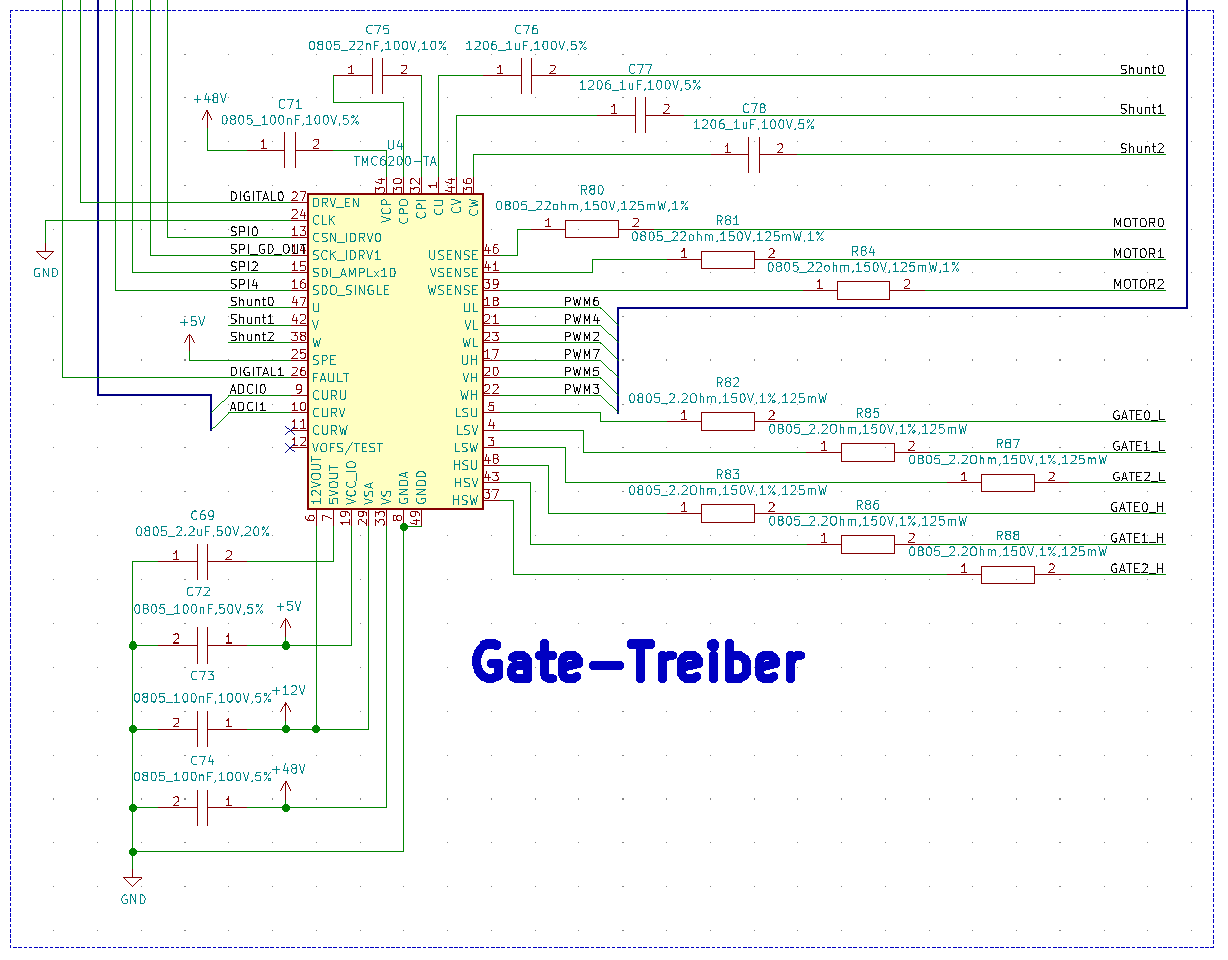
\includegraphics[width=\textwidth]{graphics/Schema_Gate_Treiber}
	\caption{Schema Gate-Treiber.}
	\label{fig:Schema_Gate_Treiber}
\end{figure}

%\begin{figure}[h!]
%	\centering
%	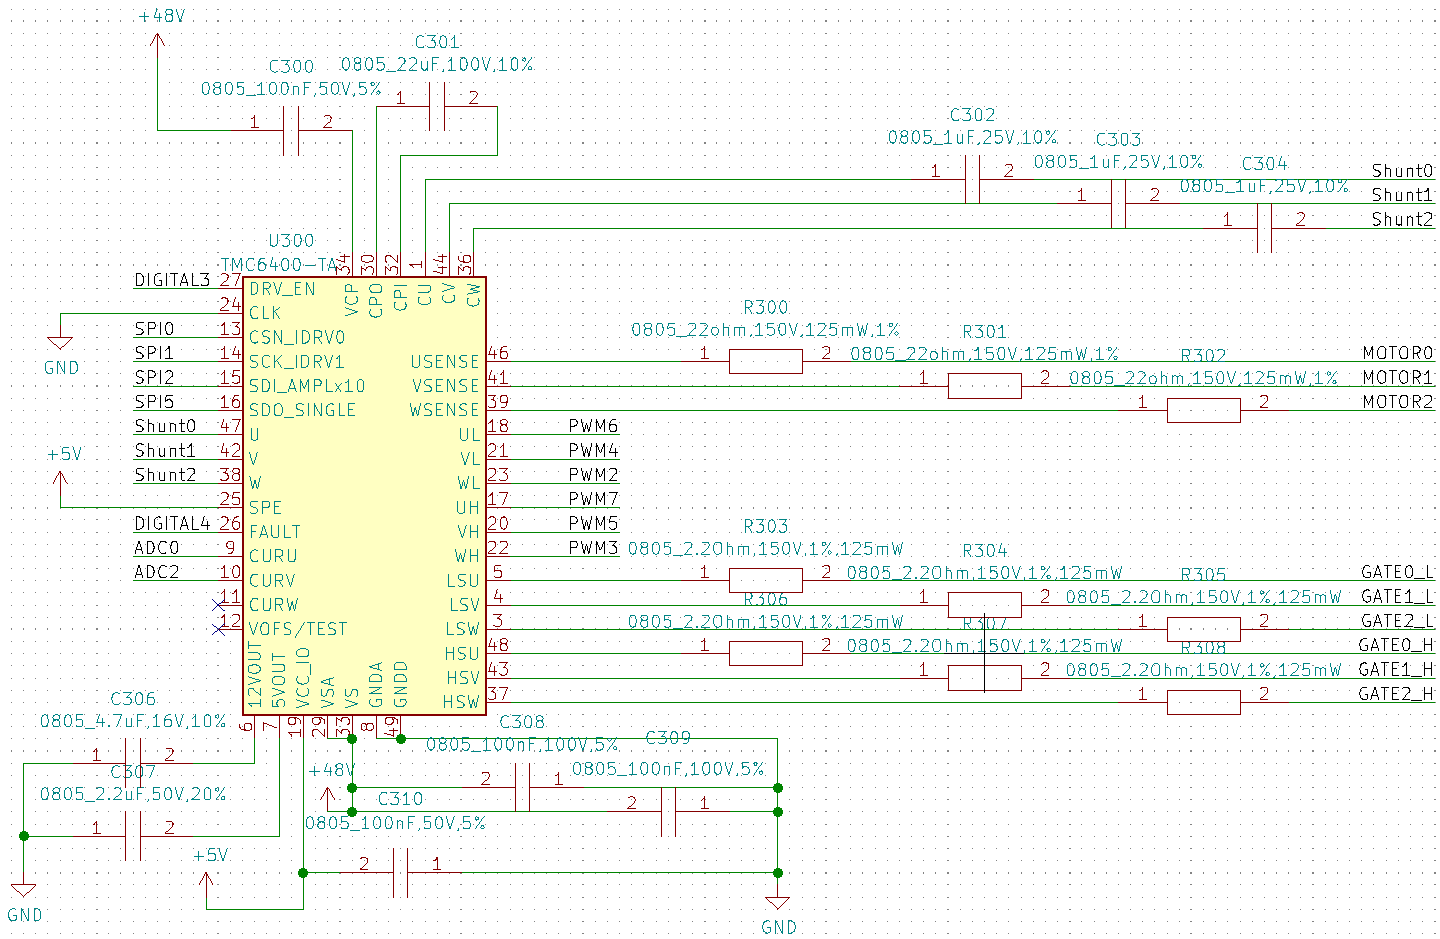
\includegraphics[width=0.8\textwidth]{graphics/TMC6200_Schema.png}
%	\caption{Teilschema Ansteuerung Motor. Hier Gate-Treiber-IC TMC6200.}
%	\label{fig:Schema_TMC6200}
%\end{figure}
%\begin{figure}[h!]
%	\centering
%	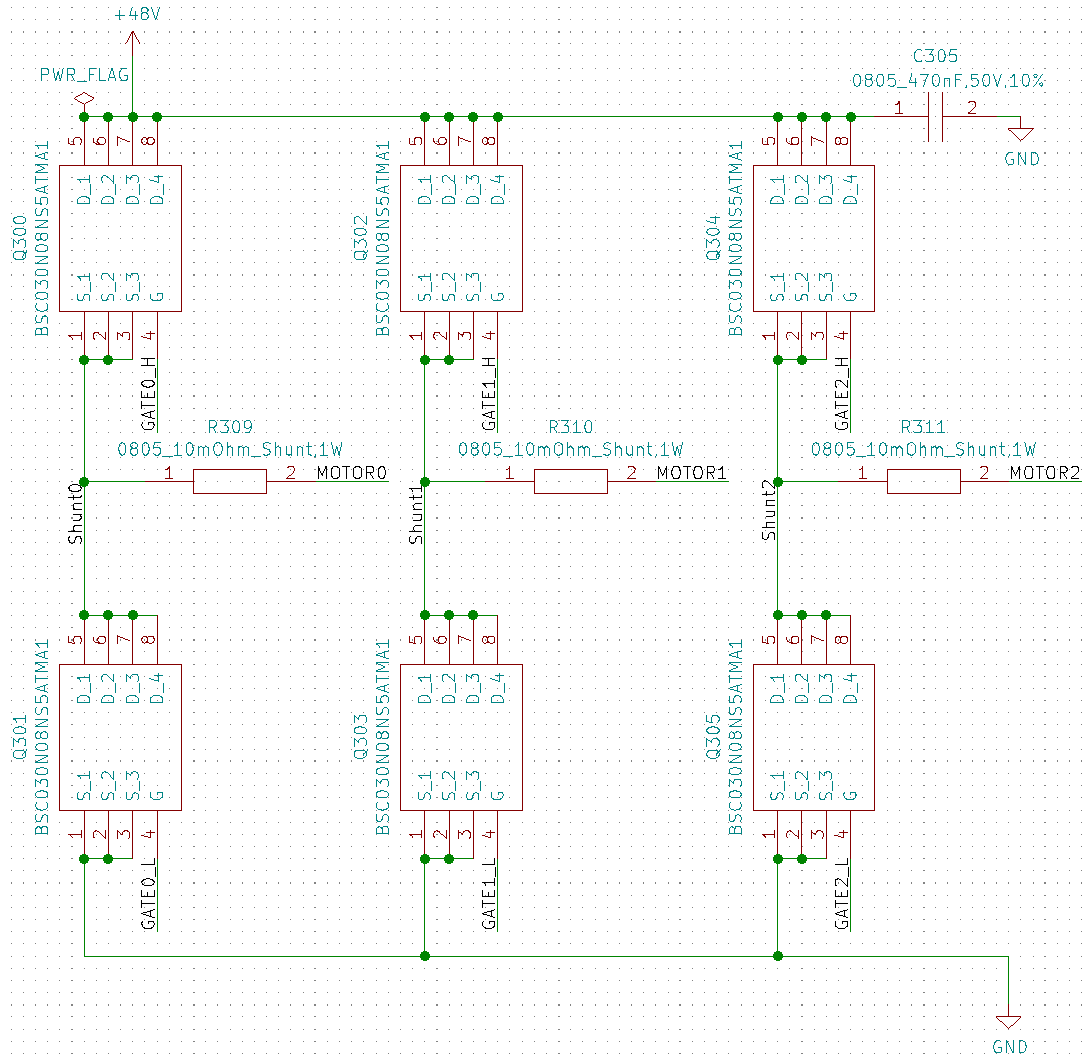
\includegraphics[width=0.6\textwidth]{graphics/H_Bruecke_Schema.png}
%	\caption{Teilschema Ansteuerung Motor. Hier H-Brücke.}
%	\label{fig:Schema_TMC6200}
%\end{figure}

Im Schema sind die Korrekturen Rot gekennzeichnet. Im Layout wurden die Pins fälschlicherweise vertauscht. Weiter ist zu beachten, dass die Gate-Treiber-Schaltung sich nicht mehr auf der Leiterplatine befindet, sondern auf einem externen Breakout-Board. Die SPI-Pins werden nicht mehr über die vorgesehenen Leitungen angesteuert, sondern über die ursprünglichen Header-Pins des FOC-Treibers.

\paragraph{Funktionsbeschrieb der Schaltung}\mbox{}

%\subparagraph{Shunt-Widerstände $\mathrm{\mathbf{R_{Sense}}}$}
%\begin{tabular}{lll}
%$\mathbf{R_{Sense}}$ =  \textbf{10m\textOmega}\\
%\textbf{Verstärkungsfaktor}= \textbf{10x}   
%\end{tabular}
%\paragraph{Gate Vorwiderstände $\mathrm{\mathbf{R_{Gate}}}$}
Da das Gate ein kapazitives Verhalten zeigt, ist der Strom, welcher zu Beginn ins Gate fliesst, sehr hoch. Die \textbf{Gate-Vorwiderstände} R82, R83 und R85 bis R88 in Abbildung \ref{fig:Schema_Gate_Treiber} begrenzen diesen.
Die Dimensionierung der Gate-Widerständen lehnt an die MOSFET Gate-Drain-Ladung (Miller charge) an. Aus dem Datenblatt ist einer Tabelle zu entnehmen, wie gross der Widerstand bei gegebener Miller charge sein muss. Die Tabelle mit den ermittelten Parameter ist im Anhang Kapitel \ref{Appendix:Gate_Vorwiderstand} zu finden. Die Gate-Ladung des ausgewählten MOSFET's beträgt 61nC. Gemäss der Tabelle muss der Vorwiderstand mit R$_{Gate}\leq$2.5\textOmega\ dimensioniert werden. Dies bedingt, dass programmierbare Register DRV\_STRENGTH auf 1 bis 3 gesetzt ist \cite[S.13]{trinamicmotion_control_gmbh__co_kg_tmc6200_2019}.

%\begin{tabular}{lll}
%$\mathrm{\mathbf{R_{Gate}}}$ & \textbf{=} & $\mathrm{\mathbf{R_{Gate}\leq2.5\Omega}}$ \\
%\textbf{DRV\_STRENGTH} & \textbf{=} & \textbf{1 bis 3}
%\end{tabular}

%\paragraph{Schutzwiderstände Messeingang $\mathrm{\mathbf{R_{Protect}}}$}

Wird von einem High-Zustand in einen Low-Zustand gewechselt, kann aufgrund von Induktivitäten die Spannung unterschiessen. Die \textbf{Schutzwiderstände} R80, R81 und R84 in Abbildung \ref{fig:Schema_Gate_Treiber} schützen die Messeingänge des Gate-Treibers vor diesem Effekt.
Die Dimensionierung dieses Widerstands wird im Datenblatt mit einem Widerstandswert zwischen 10\textOmega\ und 22\textOmega\ angegeben \cite[S.10]{trinamicmotion_control_gmbh__co_kg_tmc6200_2019}.

%\begin{tabular}{lll}
%$\mathrm{\mathbf{R_{P}}}$ & \textbf{=} & \textbf{10\textOmega\ bis 22\textOmega}\\
%\end{tabular}

%\paragraph{Bootstrap Kondensatoren $\mathrm{\mathbf{C_{Bootstrap}}}$}

Die \textbf{Bootstrap-Kondensatoren} C76 - C78 in Abbildung \ref{fig:Schema_Gate_Treiber} werden eingesetzt, um die Gate-Spannung am High-Side-MOSFET auf die anliegende Schaltspannung plus die Gatespannung anzuheben.
Die Dimensionierung dieser Kondensatoren wird im Datenblatt mit einem Kapazitätswert zwischen 470nF und 1\textmugreek F angegeben, bei einer Nennspannung von 16V oder 25V. Weiter gilt gemäss Datenblatt, dass bei MOSFET's mit einem $\mathrm{Q_G \geq 40nC}$ die Gatekapazität 1\textmugreek F sein soll \cite[S.10]{trinamicmotion_control_gmbh__co_kg_tmc6200_2019}. Da die Kapazität 61nF beträgt, ist dies der Fall. 

%\begin{tabular}{lll}
%$\mathrm{\mathbf{C_{Bootstrap}}}$ & \textbf{=} & \textbf{1\textmugreek F (25V)}\\
%\end{tabular}

%\paragraph{Externer Gate-Spannungsregler}

Aufgrund der hohen Versorgungsspannung (48V), treten im IC über den Gate- und 5V- Spannungsreglern erhebliche Verluste auf. Um diese Verluste zu reduzieren, wird laut Datenblatt geraten, eine externe Gate-Spannung anzuhängen. Für beste Resultate wird eine Spannung von 12V $\pm$ 1V empfohlen.
Aus dem Datenblatt des Gate-Treibers ist zu entnehmen, dass für den Kondensator C69 2.2\textmugreek F und für den Kondensator C73 100nF verwendet werden. Beide sind in Abbildung \ref{fig:Schema_Gate_Treiber} zu sehen. Der Kondensator C73 sowie die Kondensatoren C72 und C74 sind \textbf{Stützkondensatoren} und glätten die Versogrungsspannungen auf den jeweiligens Spannungsebenen.

%\begin{tabular}{lll}
%$\mathrm{\mathbf{C_{69}}}$ & \textbf{=} & \textbf{2.2\textmugreek F}\\
%$\mathrm{\mathbf{C_{73}}}$ & \textbf{=} & \textbf{100nF}\\
%\end{tabular}